\let\negmedspace\undefined
\let\negthickspace\undefined
\documentclass[journal]{IEEEtran}
\usepackage[a5paper, margin=10mm, onecolumn]{geometry}
%\usepackage{lmodern} % Ensure lmodern is loaded for pdflatex
\usepackage{tfrupee} % Include tfrupee package

\setlength{\headheight}{1cm} % Set the height of the header box
\setlength{\headsep}{0mm}     % Set the distance between the header box and the top of the text

\usepackage{gvv-book}
\usepackage{gvv}
\usepackage{cite}
\usepackage{amsmath,amssymb,amsfonts,amsthm}
\usepackage{algorithmic}
\usepackage{graphicx}
\usepackage{textcomp}
\usepackage{xcolor}
\usepackage{txfonts}
\usepackage{listings}
\usepackage{enumitem}
\usepackage{mathtools}
\usepackage{gensymb}
\usepackage{comment}
\usepackage[breaklinks=true]{hyperref}
\usepackage{tkz-euclide} 
\usepackage{listings}
% \usepackage{gvv}                                        
\def\inputGnumericTable{}                                 
\usepackage[latin1]{inputenc}                                
\usepackage{color}                                            
\usepackage{array}                                            
\usepackage{longtable}                                       
\usepackage{calc}                                             
\usepackage{multirow}                                         
\usepackage{hhline}                                           
\usepackage{ifthen}                                           
\usepackage{lscape}
\usepackage{circuitikz}


\renewcommand{\thefigure}{\theenumi}
\renewcommand{\thetable}{\theenumi}
\setlength{\intextsep}{10pt} % Space between text and floats


\numberwithin{equation}{enumi}
\numberwithin{figure}{enumi}
\renewcommand{\thetable}{\theenumi}


% Marks the beginning of the document
\begin{document}
\bibliographystyle{IEEEtran}
\vspace{3cm}

\title{GATE 2010 EE(40-52)}
\author{EE24BTECH11030 - J.KEDARANANDA}
% \maketitle
% \newpage
% \bigskip
{\let\newpage\relax\maketitle}
\renewcommand{\thefigure}{\theenumi}
\renewcommand{\thetable}{\theenumi}
\begin{enumerate}
    \item A separately excited DC machine is coupled to a 50 Hz, three-phase, 4-pole induction machine as shown in the figure. The DC machine is energized first and the machines rotate at 1600 rpm. Subsequently, the induction machine is also connected to a 50 Hz, three-phase source, the phase sequence being consistent with the direction of rotation. In steady state,

    \begin{figure}[!ht]
\centering
\resizebox{\textwidth}{!}{%
\begin{circuitikz}
\ctikzset{bipoles/length=1cm, font=\LARGE}
\draw (8,19) to[short] (8,19);
\draw (9,18) to[short] (11,18);
\draw (11,18) to[short] (13,18);
\draw (9,15.25) to[short] (13,15.25);
\draw (9,18) to[short] (9,17);
\draw (13,18) to[short] (13,17.5);
\draw (13.5,16.5) to[short] (15.75,16.5);
\draw (13.5,17) to[short] (15.75,17);
\draw (18.25,17.75) to[short] (20.25,17.75);
\draw (18.5,16.75) to[short] (20.5,16.75);
\draw (18.25,15.75) to[short] (20.5,15.75);
\draw (20.25,17.75) to[short] (21.5,19);
\draw (20.75,16) to[short] (20.75,18.25);
\draw (20.5,16.75) to[short] (21.75,18);
\draw (20.5,15.75) to[short] (22,17.25);
\draw (17.75,17.25) to[short] (18.25,17.75);
\draw (17.75,16.75) to[short] (18.5,16.75);
\draw (17.75,16.25) to[short] (18.25,15.75);
\draw (13,16.75) circle (0.5cm);
\draw (16.75,16.75) circle (1cm);
\draw (9,17) to[battery1] (9,15.25);
\draw (13,16) to[short] (13,15.25);
\draw (21,16.25) to[short] (21,18.5);
\filldraw [fill={rgb,255:red,27; green,24; blue,24}] (12.75,17.5) rectangle (13.25,17.25);
\filldraw [fill={rgb,255:red,16; green,15; blue,15}] (12.75,16.25) rectangle (13.25,16);
\draw [short] (10,16) -- (10,17);
\draw (10,17) to[R] (12,17);
\draw (10,16) to[battery1] (12,16);
\draw (12,16) to[short] (12,17);
\node at (12.25,18.5) {DC machine};
\node at (17.25,18.75) {Induction machine};
\node at (17.25,18.25) {4 pole, 50Hz};
\node at (26,17.75) {50Hz balanced};
\node at (26,17.25) {3 phase supply};
\draw (23.25,18) to[short] (24.5,18);
\draw (23.25,17.5) to[short] (24.5,17.5);
\draw (23.25,17) to[short] (24.5,17);
\draw [->, >=Stealth] (22.25,18) -- (23,17.5);
\draw [->, >=Stealth] (14.75,17.25) .. controls (15.25,17.25) and (15.25,16.75) .. (14.75,16.25);
\end{circuitikz}
}%
\caption{}
\label{fig:1}
\end{figure}
    \begin{enumerate}
        \item both machines act as generators
        \item the DC machine acts as a generator, and the induction machine acts as a motor
        \item the DC machine acts as a motor, and the induction machine acts as a generator
        \item both machines act as motors
    \end{enumerate}

    \item A balanced star-connected and purely resistive load is connected at the secondary of a star-delta transformer as shown in the figure. The line-to-line voltage rating of the transformer is 110 V / 220 V. Neglecting the non-idealities of the transformer, the impedance $Z$ of the equivalent star-connected load, referred to the primary side of the transformer, is:

    \begin{figure}[!ht]
\centering
\resizebox{\textwidth}{!}{%
\begin{circuitikz}
\ctikzset{bipoles/length=1cm, font=\LARGE}
\draw (6,19.75) to[short] (6,19.75);
\draw (5.75,19.25) to[short] (7.75,19.25);
\draw (7.75,19.25) to[short] (10.75,19.25);
\draw (5.75,17.5) to[short] (8,17.5);
\draw (8,17.5) to[short] (10,17.5);
\draw (5.75,16.25) to[short] (8,16.25);
\draw (8,16.25) to[short] (11.5,16.25);
\draw (11.5,16.25) to[short] (11.5,17.5);
\draw (10,17.5) to[L] (10.75,18.25);
\draw (10.75,18.25) to[L] (11.5,17.5);
\draw (10.75,19.25) to[L] (10.75,18.25);
\draw (5.75,15.25) to[short] (11.25,15.25);
\draw (5.75,12.5) to[short] (10,12.5);
\draw (5.75,11.5) to[short] (12.5,11.5);
\draw (12.5,11.5) to[short] (12.5,12.5);
\draw (11.25,15.25) to[european resistor] (11.25,13.75);
\draw (10,12.5) to[european resistor] (11.25,13.75);
\draw (11.25,13.75) to[european resistor] (12.5,12.5);
\draw (16.75,19.25) to[short] (21.75,19.25);
\draw (18.25,17.75) to[short] (20.25,17.75);
\draw (16.75,16.25) to[short] (23.25,16.25);
\draw (16.75,16.25) to[L] (16.75,19.25);
\draw (16.75,16.25) to[L] (18.25,17.75);
\draw (16.75,19.25) to[L] (18.25,17.75);
\draw (21.75,19.25) to[R] (21.75,17.75);
\draw (19.75,17.75) to[R] (21.75,17.75);
\draw (21.75,17.75) to[R] (23.25,16.25);

\node at (5.25,15) {R};
\node at (5.25,17.75) {Y};
\node at (5.25,16.25) {B};
\node at (5.25,19.25) {R};
\node at (5.25,12.75) {Y};
\node at (5.25,11.5) {B};
\node at (12.25,13.5) {Z};
\node at (10.75,14.5) {Z};
\node at (10.75,12.5) {Z};
\node at (23.25,17.5) {4$\Omega$};
\node at (21,18.5) {4$\Omega$};
\node at (21,17) {4$\Omega$};
\node at (19,19.75) {r};
\node at (19,18) {b};
\node at (19,16.75) {y};
\end{circuitikz}
}%
\end{figure}
\newpage

    \begin{enumerate}
        \item $3 + j 0$ $\Omega$
        \item $0.866 - j 0.5$ $\Omega$
        \item $0.866 + j 0.5$ $\Omega$
        \item $1 + j 0$ $\Omega$
    \end{enumerate}

    \item Consider a three-phase, 50 Hz, 11 kV distribution system. Each of the conductors is suspended by an insulator string having two identical porcelain insulators. The self-capacitance of the insulator is 5 times the shunt capacitance between the link and the ground, as shown in the figure. The voltage across the two insulators are:
    \begin{figure}[!ht]
\centering
\resizebox{0.6\textwidth}{0.4\textheight}{%
\begin{circuitikz}[scale=1]
\ctikzset{bipoles/length=1cm, font=\LARGE}
\draw (9.75,19.5) to[short] (9.75,19.5);
\draw (9.75,19.75) to[short] (12.75,19.75);
\draw (9.75,19.75) to[short] (9.75,16.75);
\draw (9.75,19.75) to[short] (10.25,20.25);
\draw (10.5,19.75) to[short] (11,20.25);
\draw (11.25,19.75) to[short] (11.75,20.25);
\draw (12,19.75) to[short] (12.5,20.25);
\draw (9.25,19) to[short] (9.75,19.5);
\draw (9.25,18.25) to[short] (9.75,18.75);
\draw (9.25,17.5) to[short] (9.75,18);
\draw (9.25,16.75) to[short] (9.75,17.25);
\draw (12,18.5) to[short] (12.75,18.5);
\draw (9.75,18.5) to[C] (11.25,18.5);
\draw (11.25,19.75) to[C] (11.25,18.5);
\draw (11.25,18.5) to[C] (11.25,16.75);
\draw (11.25,17) circle (0cm);
\draw [->, >=Stealth] (12.75,19.25) -- (12.75,19.75);
\draw [->, >=Stealth] (12.75,18.75) -- (12.75,18.5);
\draw [->, >=Stealth] (12.75,18) -- (12.75,18.5);
\draw [->, >=Stealth] (12.75,17.5) -- (12.75,16.75);

\node [font=\normalsize] at (12.75,19) {$e_1$};
\node [font=\normalsize] at (12.75,17.75) {$e_2$};
\node [font=\LARGE] at (10,18) {C};
\node [font=\LARGE] at (12,19.25) {5C};
\node [font=\LARGE] at (10.75,17.25) {5C};
\end{circuitikz}
}%
\end{figure}


    \begin{enumerate}
        \item $e_1 = 3.74$ kV, $e_2 = 2.61$ kV
        \item $e_1 = 3.46$ kV, $e_2 = 2.89$ kV
        \item $e_1 = 6.0$ kV, $e_2 = 4.23$ kV
        \item $e_1 = 5.5$ kV, $e_2 = 5.5$ kV
    \end{enumerate}
\item Consider a three-core, three-phase, 50 Hz, 11 kV cable whose conductors are denoted as R, Y, and B in the figure. The inter-phase capacitance ($C_1$) between each pair of conductors is 0.2 $\mu$F and the capacitance between each line conductor and the sheath is 0.4 $\mu$F. The per-phase charging current is
\begin{figure}[!ht]
\centering
\resizebox{0.6\textwidth}{!}{% Adjust the width here
\begin{circuitikz}
\tikzstyle{every node}=[font=\small]

\draw  (2.5,9) circle (2cm);

\draw (2.5,11) to[C] (2.5,9.75);

\draw  (2.5,9.5) circle (0.25cm);
\node [font=\small] at (2.5,9.5) {R};

\draw (2.25,9.5) to[C] (1.5,8.75);

\draw  (1.5,8.5) circle (0.25cm);
\node [font=\small] at (1.5,8.5) {B};

\draw (1.25,8.5) to[C] (0.75,8); 

\draw (2.25,5.25) to[short] (2.5,5.25);

\draw (3.25,8.5) to[C] (1.75,8.5);
\draw  (3.5,8.5) circle (0.25cm);
\node [font=\small] at (3.5,8.5) {Y};

\draw (3.5,8.75) to[C] (2.75,9.5);
\draw (4.25,8) to[C] (3.75,8.5);

\draw [->, >=Stealth] (3.25,7) -- (3.5,6.75);
\node [font=\normalsize] at (4.25,6.5) {Outer Sheath};

\node [font=\small] at (3.25,10.25) {C2}; 
\node [font=\small] at (3.6,7.75) {C2};
\node [font=\small] at (1.4,7.75) {C2};
\node [font=\small] at (2.5,7.75) {C1};
\node [font=\small] at (3.75,9.5) {C1};
\node [font=\small] at (1.25,9.5) {C1};

\end{circuitikz}
}%
\end{figure}

\begin{multicols}{4}
\begin{enumerate}
    \item 2.0 A
    \item 2.4 A
    \item 2.7 A
    \item 3.5 A
\end{enumerate}
\end{multicols}
\bigskip
\item  For the power system shown in the figure below$\ref{fig:5q}$, the specifications of the components are as follows:

\begin{itemize}
    \item $G_1$: 25 kV, 100 MVA, $X = 9\%$
    \item $G_2$: 25 kV, 100 MVA, $X = 9\%$
    \item $T_1$: 25 kV/220 kV, 90 MVA, $X = 12\%$
    \item $T_2$: 220 kV/25 kV, 90 MVA, $X = 12\%$
    \item Line 1: 220 kV, $X = 150$ ohms
\end{itemize}
\begin{figure}[!ht]
    \centering
    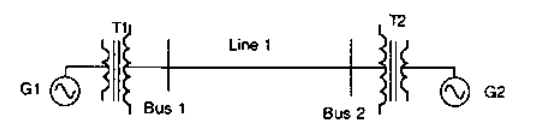
\includegraphics[scale=0.4]{figs/5q.png}
    \caption{}
    \label{fig:5q}
\end{figure}
\noindent Choose $25 \, \text{kV}$ as the base voltage at generator $G_1$, and $200 \, \text{MVA}$ as the MVA base. The impedance diagrams are shown below:
\begin{enumerate}
    \item 
    \begin{figure}[!ht]
        \centering
        \resizebox{1\textwidth}{!}{
            \begin{circuitikz}
                \tikzstyle{every node}=[font=\small]
                \draw (1.25,9.5) to[L, l=$j0.18$] (1.25,8.25);
                \draw (1.25,9.5) to[L, l=$j0.27$] (3,9.5);
                \draw (3,9.5) to[L, l=$j0.42$] (4.75,9.5);
                \draw (4.75,9.5) to[L, l=$j0.27$] (6.5,9.5);
                \draw (6.5,9.5) to[L, l=$j0.18$] (6.5,8.25);
                \draw (6.5,8.25) to[sinusoidal voltage source, l={G2}] (6.5,7.25);
                \draw (6.5,7.25) to[short] (1.25,7.25);
                \draw (1.25,8.25) to[sinusoidal voltage source, l={G1}] (1.25,7.25);
                \draw [line width=1pt] (3,10) to[short] (3,9.25);
                \draw [line width=1pt] (4.75,10) to[short] (4.75,9.25);
            \end{circuitikz}
        }
    \end{figure}

    \item 
    \begin{figure}[!ht]
        \centering
        \resizebox{1\textwidth}{!}{
            \begin{circuitikz}
                \tikzstyle{every node}=[font=\small]
                \draw (1.25,9.5) to[L, l=$j0.18$] (1.25,8.25);
                \draw (1.25,9.5) to[L, l=$j0.27$] (3,9.5);
                \draw (3,9.5) to[L, l=$j0.62$] (4.75,9.5);
                \draw (4.75,9.5) to[L, l=$j0.27$] (6.5,9.5);
                \draw (6.5,9.5) to[L, l=$j0.18$] (6.5,8.25);
                \draw (6.5,8.25) to[sinusoidal voltage source, l={G2}] (6.5,7.25);
                \draw (6.5,7.25) to[short] (1.25,7.25);
                \draw (1.25,8.25) to[sinusoidal voltage source, l={G1}] (1.25,7.25);
                \draw [line width=1pt] (3,10) to[short] (3,9.25);
                \draw [line width=1pt] (4.75,10) to[short] (4.75,9.25);
            \end{circuitikz}
        }
    \end{figure}
\newpage
    \item 
    \begin{figure}[!ht]
        \centering
        \resizebox{1\textwidth}{!}{
            \begin{circuitikz}
                \tikzstyle{every node}=[font=\small]
                \draw (1.25,9.5) to[L, l=$j0.21$] (1.25,8.25);
                \draw (1.25,9.5) to[L, l=$j0.27$] (3,9.5);
                \draw (3,9.5) to[L, l=$j0.42$] (4.75,9.5);
                \draw (4.75,9.5) to[L, l=$j0.27$] (6.5,9.5);
                \draw (6.5,9.5) to[L, l=$j0.21$] (6.5,8.25);
                \draw (6.5,8.25) to[sinusoidal voltage source, l={G2}] (6.5,7.25);
                \draw (6.5,7.25) to[short] (1.25,7.25);
                \draw (1.25,8.25) to[sinusoidal voltage source, l={G1}] (1.25,7.25);
                \draw [line width=1pt] (3,10) to[short] (3,9.25);
                \draw [line width=1pt] (4.75,10) to[short] (4.75,9.25);
            \end{circuitikz}
        }
    \end{figure}

    \item 
    \begin{figure}[!ht]
        \centering
        \resizebox{1\textwidth}{!}{
            \begin{circuitikz}
                \tikzstyle{every node}=[font=\small]
                \draw (1.25,9.5) to[L, l=$j0.21$] (1.25,8.25);
                \draw (1.25,9.5) to[L, l=$j0.3$] (3,9.5);
                \draw (3,9.5) to[L, l=$j0.42$] (4.75,9.5);
                \draw (4.75,9.5) to[L, l=$j0.3$] (6.5,9.5);
                \draw (6.5,9.5) to[L, l=$j0.21$] (6.5,8.25);
                \draw (6.5,8.25) to[sinusoidal voltage source, l={G2}] (6.5,7.25);
                \draw (6.5,7.25) to[short] (1.25,7.25);
                \draw (1.25,8.25) to[sinusoidal voltage source, l={G1}] (1.25,7.25);
                \draw [line width=1pt] (3,10) to[short] (3,9.25);
                \draw [line width=1pt] (4.75,10) to[short] (4.75,9.25);
            \end{circuitikz}
        }
    \end{figure}
\end{enumerate}
\bigskip
\item
The TTL circuit shown in the figure $\ref{fig:46q}$is fed with the waveform $X$ (also shown). All gates have equal propagation delay of $10 \, \text{ns}$. The output $Y$ of the circuit is
\begin{figure}[!ht]
\centering
\resizebox{1\textwidth}{!}{%
\begin{circuitikz}
\tikzstyle{every node}=[font=\large]
\draw (10.5,19.5) to[short] (10.5,19.5);
\draw (10.75,19.25) to[short] (17.75,19.25);
\draw (11.25,19.25) to[short] (11.25,17.5);
\draw (15.75,17.75) to[short] (15.75,17.25);
\draw (13,17.75) to[short] (13,17.25);
\draw (17.75,19.25) to[short] (18,19.25);
\draw (17.75,18.75) to[short] (18,18.75);
\draw (18,19.25) node[ieeestd xor port, anchor=in 1, scale=0.89](port){} (port.out) to[short] (19.75,19);
\draw (13,17.75) to[short] (13.25,17.75);
\draw (13,17.25) to[short] (13.25,17.25);
\draw (13.25,17.75) node[ieeestd nand port, anchor=in 1, scale=0.89](port){} (port.out) to[short] (15,17.5);
\draw (15.75,17.75) to[short] (16,17.75);
\draw (15.75,17.25) to[short] (16,17.25);
\draw (16,17.75) node[ieeestd nand port, anchor=in 1, scale=0.89](port){} (port.out) to[short] (17.75,17.5);
\draw (11.25,17.5) to[short] (13,17.5);
\draw (15,17.5) to[short] (15.75,17.5);
\draw (17.75,17.5) to[short] (17.75,18.75);
\node [font=\large] at (10.25,19.25) {$X$};
\node [font=\large] at (20,19) {$Y$};
\end{circuitikz}
}%
\end{figure}
\newpage
\begin{figure}[!ht]
    \centering
    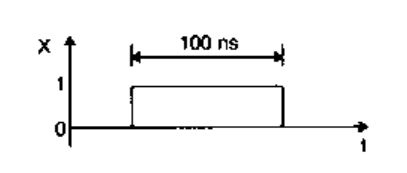
\includegraphics[scale=0.5]{figs/46q.png}
    \caption{}
    \label{fig:46q}
\end{figure}
\begin{enumerate}
    \item \begin{figure}[!ht]
         \centering
         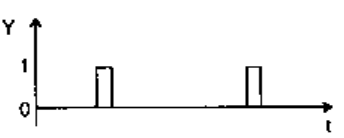
\includegraphics[scale=0.4]{figs/46a.png}
         \end{figure}
    \item \begin{figure}[!ht]
         \centering
         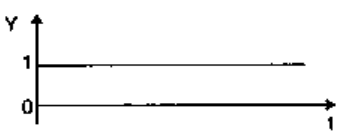
\includegraphics[scale=0.4]{figs/46b.png}
         \end{figure}
    \item \begin{figure}[!ht]
         \centering
         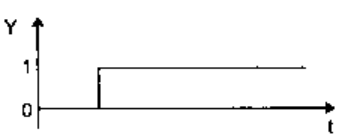
\includegraphics[scale=0.4]{figs/46c.png}
         \end{figure}
    \item \begin{figure}[!ht]
         \centering
         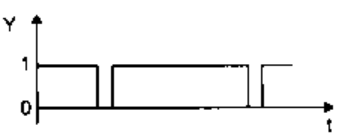
\includegraphics[scale=0.4]{figs/46d.png}
         \end{figure}
\end{enumerate}
\bigskip
\item
When a $\text{CALL Addr}$ instruction is executed, the CPU carries out the following sequential operations internally:

\begin{multicols}{2}
\begin{enumerate}
    \item  
        
            $(\text{SP})$ incremented \\
            $(\text{PC}) \leftarrow \text{Addr}$ \\
            $((\text{SP})) \leftarrow (\text{PC})$ \\
        
    \item  
        
            $(\text{PC}) \leftarrow \text{Addr}$ \\
            $((\text{SP})) \leftarrow (\text{PC})$ \\
            $(\text{SP})$ incremented \\
        
    \item  
        
            $(\text{PC}) \leftarrow \text{Addr}$ \\
            $(\text{SP})$ incremented \\
            $\leftarrow (\text{PC})$ \\
        
    \item  
        
            $((\text{SP})) \leftarrow (\text{PC})$ \\
            $(\text{SP})$ incremented \\
            $(\text{PC}) \leftarrow \text{Addr}$ \\
\end{enumerate}
\end{multicols}
\textbf{COMMON DATA QUESTIONS}\\
\textbf{COMMON DATA FOR QUESTIONS 48 AND 49}\\\\
A separately excited DC motor runs at 1500 rpm under no-load with 200 V applied to the armature. The field voltage is maintained at its rated value. The speed of the motor, when it delivers a torque of 5 Nm, is 1400 rpm as shown in the figure.$\ref{fig:48,49}$ The rotational losses and armature reaction are neglected.
\begin{figure}[!ht]
    \centering
    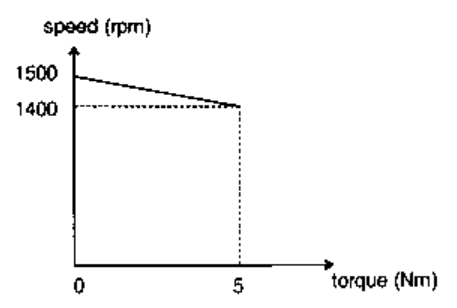
\includegraphics[scale=0.4]{figs/48,49.png}
    \caption{}
    \label{fig:48,49}
\end{figure}
\item
The armature resistance of the motor is:

\begin{multicols}{4}
\begin{enumerate}
    \item $2 \, \Omega$
    \item $3.4 \, \Omega$
    \item $4.4 \, \Omega$
    \item $7.7 \, \Omega$
\end{enumerate}
\end{multicols}

\item
For the motor to deliver a torque of $2.5 \, \text{Nm}$ at $1400 \, \text{rpm}$, the armature voltage to be applied is:

\begin{multicols}{4}
\begin{enumerate}
    \item $125.5 \, \text{V}$
    \item $193.3 \, \text{V}$
    \item $210 \, \text{V}$
    \item $241.7 \, \text{V}$
\end{enumerate}
\end{multicols}
\newpage
\textbf{COMMON DATA FOR QUESTIONS 50 AND 51}\\
\textbf{Given $f(t)$ and $g(t)$ as shown below:\ref{fig:50,51}}\\\\
\begin{figure}[!ht]
    \centering
    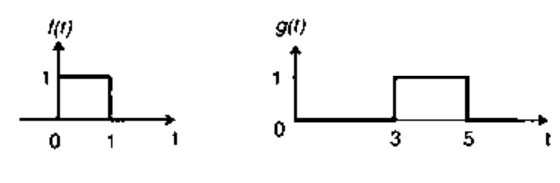
\includegraphics[scale=0.4]{figs/50,51.png}
    \caption{}
    \label{fig:50,51}
\end{figure}
\item $g(t)$ can be expressed as

\begin{multicols}{2}
\begin{enumerate}
    \item $g(t) = f(2t - 3)$
    \item $g(t) = f\left(\frac{t}{2} - 3\right)$
    \item $g(t) = f\left(2 - \frac{3}{2}\right)$
    \item $g(t) = f\left(\frac{t}{2} - \frac{3}{2}\right)$
\end{enumerate}
\end{multicols}
\item  The Laplace transform of $g(t)$ is
    \begin{enumerate}
    \begin{multicols}{2}
        \item $\frac{1}{s} \left(e^{a} - e^{b}\right)$
        \item $\frac{1}{s} \left(e^{a} - e^{c}\right)$
        \item $\frac{e^{b}}{s} \left(1 - e^{-a}\right)$
        \item $\frac{1}{s} \left(e^{a} - e^{c}\right)$
    \end{multicols}
    \end{enumerate}

\bigskip

\textbf{Linked Answer Questions}\\
\textbf{Statement for Linked Answer Questions 52 and 53:} \\\\
The following Karnaugh map $\ref{fig:52}$ represents a function $F$.
\begin{figure}[!ht]
    \centering
    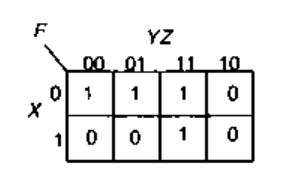
\includegraphics[scale=0.4]{figs/52.png}
    \caption{}
    \label{fig:52}
\end{figure}
\item  A minimized form of the function $F$ is
    \begin{enumerate}
    \begin{multicols}{2}
        \item $F = \overline{X}Y + YZ$
        \item $F = \overline{X}\overline{Y} + YZ$
        \item $F = \overline{X}Y + \overline{Z}$
        \item $F = \overline{X}\overline{Y} + \overline{Z}$
    \end{multicols}
    \end{enumerate}
\end{enumerate}
\end{document}




